\subsection{Đường quét bao phủ kiểu tiến - lui RCPP}
\label{sec:sea}
Phương pháp RCPP gồm ba bước như sau:
\begin{itemize}
    \item \textbf{Bước 1: Tìm các cặp cạnh đối đỉnh}
    
    Các cặp đối đỉnh là các cặp đỉnh của đa giác mà cho phép các đường hỗ trợ song song giao với ranh giới của đa giác và nằm hoàn toàn về một phía của nó. Chúng có thể được xác định bằng thuật toán của Shamon \cite{shamos1978computational}.

Ở phần này, vấn đề sẽ được giải quyết từ góc độ 2D, do đó không gian làm việc sẽ là không gian hai chiều và nó sẽ được gọi là robot. Một điểm trên không gian làm việc được xác định bởi một cặp giá trị $(x, y)$. Cho rằng vùng quan tâm (ROI) là mặt phẳng, vì vậy nó được biểu thị bằng một hình đa giác lồi dạng tiêu chuẩn (convext) \cite{10.1007/11841036_57}, $Q = \{ V, E \}$. Trong đó $V$ là tập hợp các đỉnh, điểm trong cùng một mặt phẳng đặt theo chiều kim đồng hồ. $E$ là tập hợp các cạnh tạo bởi 2 điểm liên tiếp nhau.

Ta sẽ định nghĩa đường hỗ trợ là một đường thẳng đi qua 1 đỉnh của đa giác hoặc 1 cạnh của đa giác và nằm hoàn toàn về một phía của đa giác, không cắt đa giác tại điểm nào. Một cặp điểm đối đỉnh là 1 cặp điểm mà ở 2 điểm đó tồn tại 2 đường hỗ trợ đi qua và song song với nhau và khoảng cách giữa 2 đường thẳng song song chính là chiều rộng của đa giác.

Nhiệm vụ khảo sát được thực hiện bởi một robot mang một máy ảnh có khả năng bao phủ được một vùng. Robot được xác định là một điểm $P = (X, Y)$, trong đó X và Y là tọa độ NED. Khi robot bao phủ một khu vực, nó xuất phát tại điểm PS, di chuyển đến khu vực quan tâm, đi theo một con đường trong khi nó chụp ảnh và cuối cùng di chuyển đến điểm kết thúc, PE. Cho rằng một bức tranh được chụp từ máy ảnh có thể chụp được một hình chữ nhật trên mặt đất.

Đường kính của hình đa giác lồi là khoảng cách lớn nhất giữa các đường hỗ trợ song song. Nhìn vào Hình \ref{fig:anh1} và lưu ý rằng các đường hỗ trợ song song không thể được thực hiện để vượt qua từng cặp điểm. Ví dụ, không có đường hỗ trợ nào đi qua các đỉnh D và F có thể song song với nhau. Điều này có nghĩa là DF không phải là đường kính. Một cặp điểm tồn tại các đường hỗ trợ song song sẽ được gọi là cặp đối đỉnh. Vì vậy chúng ta chỉ cần xem xét các cặp đối đỉnh. Vấn đề là làm sao để tìm thấy chúng mà không kiểm tra tất cả các cặp điểm.

    \begin{figure}[H]
        \centering
        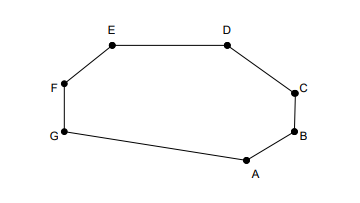
\includegraphics[width=0.6\textwidth]{chapter4/image/anh1.png}
        \caption{Hình Polygon}
        \label{fig:anh1}
    \end{figure}

\textit{Phương pháp tìm cặp điểm đối đỉnh}
\begin{itemize}
\item Quá trình thứ 1: Quay theo cùng chiều kim đồng hồ:
    Nhìn vào Hình \ref{fig:anh2}, quan sát rằng các đường thẳng L và N là các đường hỗ trợ song song thông qua các đỉnh A và D, tương ứng. Điều này có nghĩa là (A,D) là một cặp đối đỉnh nhau. Khi ta bắt đầu tiến hành quay đường hỗ trợ đồng thời theo chiều kim đồng hồ về các đỉnh này, chúng vẫn là các đường hỗ trợ. Điều này vẫn đúng cho đến khi một trong các đường hỗ trợ trở nên trùng hợp với một cạnh của đa giác. Ở đây L, khi được xoay vào vị trí L', sẽ chạm vào cạnh DE trước khi N đến B. Vì vậy (A, E) trở thành một cặp đối đỉnh. Tiếp tục theo cách này, chắc chắn sẽ tìm ra được tất cả các cặp chống đối, vì các đường song song sẽ di chuyển qua tất cả các góc có thể. Xác định cặp mới ở mỗi bước chỉ liên quan đến một so sánh góc đơn giản.
    \begin{figure}[H]
        \centering
        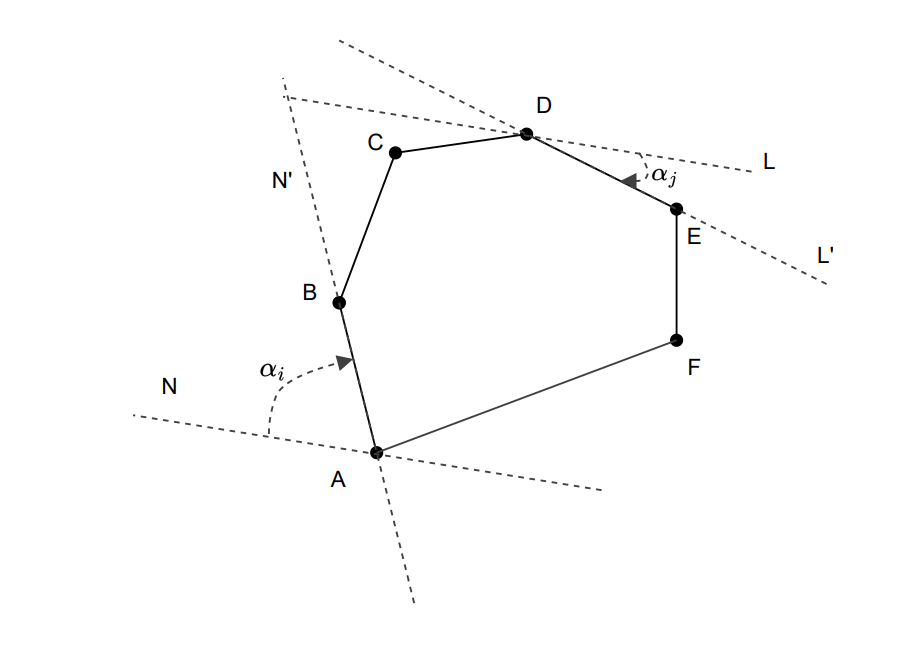
\includegraphics[width=0.8\textwidth]{chapter4/image/anh2.png}
        \caption{Xác định cặp đối đỉnh theo chiều thuận kim đồng hồ}
        \label{fig:anh2}
    \end{figure}

     Từ hình \ref{fig:anh2}, bằng cách tìm góc tối thiểu giữa $\alpha_{i}$ và $\alpha_{j}$, là các góc từ các đường hỗ trợ ảo đến cạnh gần nhất của đa giác theo thuận chiều kim đồng hồ. Tuy nhiên, thay vì đo $\alpha_{i}$ và $\alpha_{j}$, thuật toán đã đo sự khác biệt giữa vòng quay từ dòng L đến N. Xem các dòng 1-8 của Thuật toán \ref{alg:Findpoint}. Nhìn hình \ref{fig:anh3} Góc $\gamma$ là góc giữa đường thẳng L' và K. Ta có thể thấy nếu sự khác biệt giữa 2 góc $\gamma$  trừ $\pi$ nhỏ hơn 0 thì $\alpha_{i} > \alpha_{j}$ hay cạnh DE sẽ được lấy làm cơ sở của đường dẫn. Mặt khác, nếu sự khác biệt giữa 2 góc $\gamma$  trừ $\pi$ lớn hơn 0 tức là $\alpha_{i} < \alpha_{j}$, lúc đó cạnh AB được lấy làm đường cơ sở của cạnh. Một trường hợp đặc biệt là khi cả hai góc đều bằng nhau. Trong trường hợp như vậy, số lượng đường đi là như nhau sau đó, nó không quan trọng đường cơ sở nào được chọn theo số lượng đường đi. Vì lý do này và sự đơn giản trong thuật toán, trong trường hợp các góc bằng nhau, thuật toán sẽ chọn cạnh AB làm cơ sở.
    \begin{figure}[H]
        \centering
        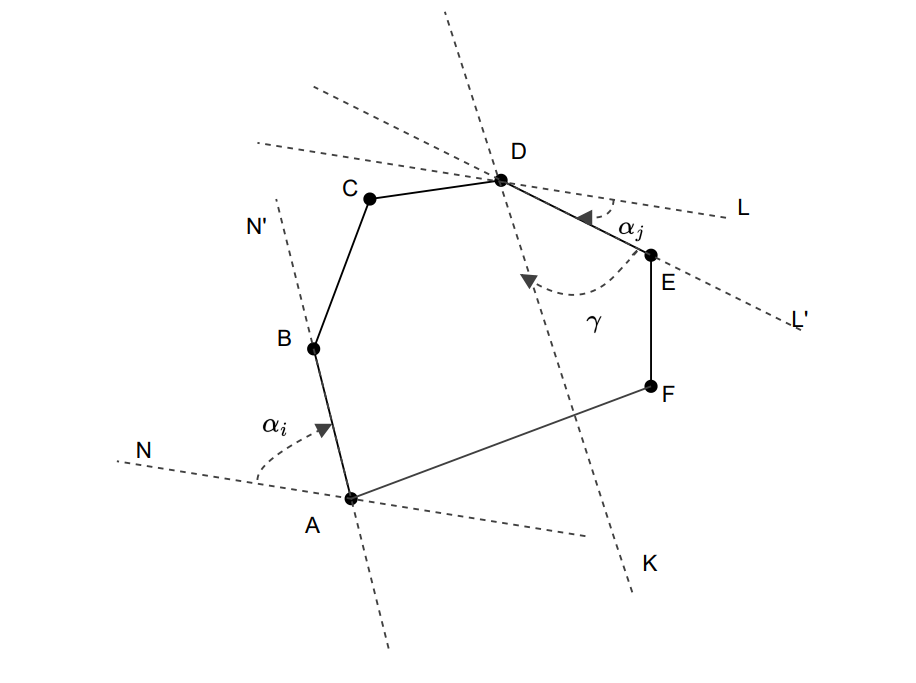
\includegraphics[width=0.8\textwidth]{chapter4/image/anh3.png}
        \caption{Xác định sự khác biệt giữa 2 góc theo chiều thuận kim đồng hồ}
        \label{fig:anh3}
    \end{figure}

    \item Quá trình thứ 2: Quay ngược chiều kim đồng hồ:
    Trong bước này, có một vài trường hợp sẽ tìm thấy đường cơ sở khác bằng cách xoay caliper theo hướng ngược chiều kim đồng hồ. Nhìn hình \ref{fig:anh4}, hai đường thẳng L,N vẫn là 2 đường thẳng hỗ trợ đi qua 2 điểm A và D. Đường thẳng H đi qua A và song song với đoạn CD. $\gamma_{a}$ là góc tạo bởi đường thằng L với cạnh CD và $\gamma_{b}$ là góc tạo bởi đường thẳng N với cạnh AF. góc $\phi$ là góc cần bổ sung để đường thẳng N có thể chạm vào cạnh AF hay $\phi= \gamma_{b}-\gamma_{a}$. Do đó ở trường hợp này đường thẳng L sẽ chạm cạnh CD trước khi đường thẳng N chạm cạnh AF. Từ đó xuất hiện một cặp đối đỉnh khác là (A,C) nếu $\gamma_{b}>\gamma_{a}$ và cặp (F,D) nếu $\gamma_{b}<\gamma_{a}$ , khác với cặp (A,E) tìm được khi quay thuận chiều kim đồng hồ. Xem dòng 7-14 từ Thuật toán \ref{alg:Findpoint}.
    
    \begin{figure}[h]
        \centering
        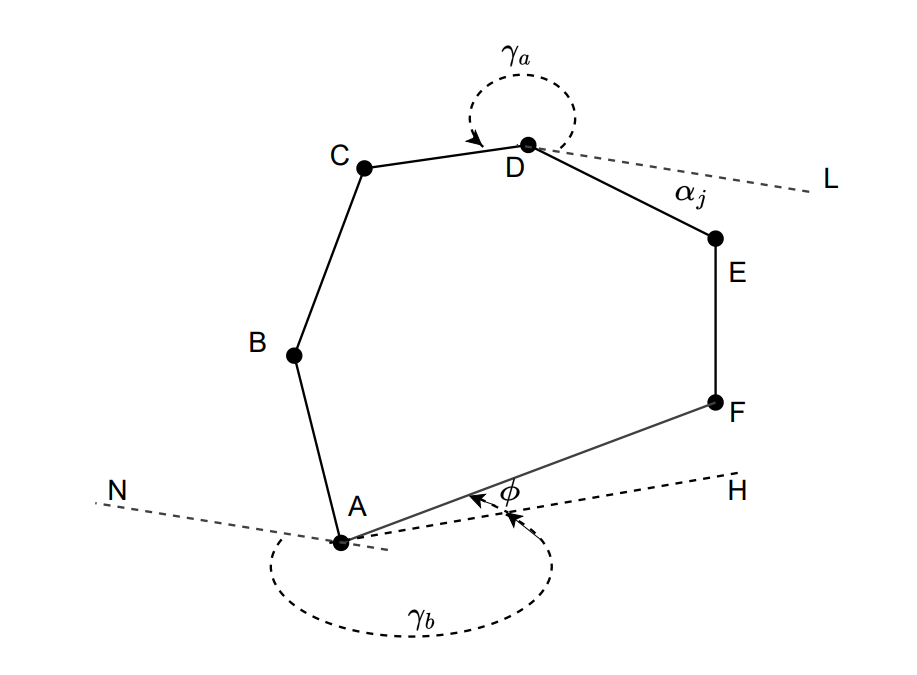
\includegraphics[width=0.7\textwidth]{chapter4/image/anh4.png}
        \caption{Xác định cặp đối đỉnh theo chiều ngược kim đồng hồ}
        \label{fig:anh4}
    \end{figure}
\end{itemize}
    Phương pháp trên có thể tóm gọn thông qua Thuật toán \ref{alg:Findpoint} như sau:

\begin{algorithm}
% \SetKwComment{Comment}{/* }{ */}
\KwData{:\textbf{V} = \{1,2,...n\} và các cặp đối đỉnh (i,j)}
\KwResult{$\rho$}
{
\tcc*[h]{Quay theo chiều thuận kim đồng hồ}\\
\If{($\text{angle}(i,j)-\pi < 0$)} 
{
    $b \gets j$\;
    $a \gets i$\;
}   
\Else
{
    $b \gets i$\;
    $a \gets j$\;
}
 \tcc*[h]{Quay ngược chiều kim đồng hồ}\\
$\gamma_{b} \gets angle(b-1,b) $\\
$\gamma_{a} \gets angle(a-1,a) $\\
    \If{$\gamma_{b} < \gamma_{a}$ }
    {
        $b_{2} \gets b-1$\\
        $a_{2} \gets a$
    }  
    \Else
    {
        $b_{2} \gets a-1$\\
        $a_{2} \gets b$
    }
}
\caption{Tìm kiếm các cặp điểm đối đỉnh}
\label{alg:Findpoint} 
\end{algorithm}

    \item \textbf{Bước 2: Tính toán đường đi tốt nhất cho từng cặp đối đỉnh}\\
    Sau khi tìm thấy tất cả các cặp đối đỉnh, đường dẫn sẽ được tạo cho từng cặp với khoảng cách tương đối là $d_x$ giữa các đường đi, $d_x = n \ell\cos{(\frac{\psi}{2})}$. 
    Đối với một cặp đối đỉnh, các đường đi được thiết kế song song với một cạnh của đa giác đi qua một trong các đỉnh của cặp đối đỉnh, còn được gọi là đường cơ sở, Đỉnh trên đường cơ sở được gọi là đỉnh bắt đầu và đỉnh còn lại được gọi là đỉnh kết thúc. Mỗi cặp đối đỉnh có hai đường cơ sở tương ứng với hai hướng cho các đường đi như trong Hình.\Ref {fig:SW1}.

    Để xây dựng đường đi bao phủ gồm các đoạn back and forth, các điểm tham chiếu vào một đường dẫn  bằng cách cho các đường đi kể trên giao nhau với đa giác Q. Thuật toán yêu cầu đầu vào là đa giác Q, đỉnh ban đầu B, một đỉnh liền kề có tên $B_{mate}$, và đỉnh đối với đỉnh B được đặt tên là A và khoảng cách giữa các đường đi là $d_x$ đã được định nghĩa bên trên.Đầu tiên, một đường đi L sẽ được tạo, song song với cạnh $( B,B_{mate}$) và phải dịch chuyển vuông góc về phía A (hướng quét) bằng cách bù, $\Delta_{init} = \dfrac{dx}{2}$

    \begin{figure}[H]
        \centering
        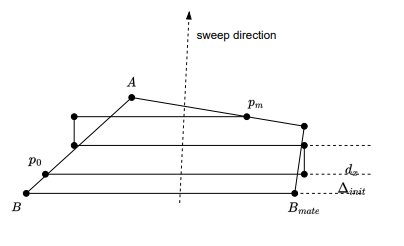
\includegraphics[width=0.7\textwidth]{chapter4/image/anh5.png}
        \caption{Xây dựng đường đi }
        \label{fig:anh5}
    \end{figure}

    Số lượng đường đi là tối thiểu nếu RCPP chọn các đường đi song song với đường cơ sở với khoảng cách tối thiểu đến đỉnh kết thúc. RCPP với các tiêu chí như vậy để chọn hướng đường đi được gọi là RCPP tối ưu, được ký hiệu là \emph{Op-RCPP}. Các đường đi song song với đường cơ sở khác được gọi là RCPP không tối ưu, được ký hiệu là \emph{nonOp-RCPP}. Như minh hoạ trong Hình. \ref{fig:SW1}, đỉnh bắt đầu là $C$ và cặp đối đỉnh là $(A,C)$. Hai đường cơ sở đi qua đỉnh $C$ là $CD$ và $CB$ với khoảng cách tương đối là $h_1$ và $h_2$ tương ứng với đỉnh kết thúc $A$. Để đạt được số lượng đường đi ít nhất, khoảng cách tương đối giữa đỉnh kết thúc và đường cơ sở phải nhỏ nhất. Trong ví dụ này, vì $h_1<h_2$, đường đi có số đường nhỏ nhất được đặt song song với $CD$.

    \item \textbf{Bước 3: Chọn một đường đi tối ưu từ tất cả các đường đi của các cặp đối đỉnh}
    
    Biểu thị $pair$ là một tập hợp các cặp đối đỉnh của đa giác. Giả sử rằng mỗi cặp đối mã $(i,j)\in pairs$ có một đường đi tốt nhất với độ dài của nó được ký hiệu là $pth_{ij}$. Gọi $ pth_{ij}^e$ là độ dài của đường đi bao gồm khoảng cách giữa điểm sao $P_s$ và đỉnh $i$, đỉnh $j$ và điểm kết thúc $P_e$. Đường dẫn tối ưu có độ dài $pth_{op}$ được chọn thỏa mãn điều kiện sau:

    \begin{equation}
        pth_{op}=pth_{op}=\min_{(i,j)\in pairs}\{pth_{ij}^{e}\text{\}}
        \label{eq:optimalpath}
    \end{equation}

    Thuật toán sẽ thực hiện so sánh tổng quãng đường mà robot đi để bao phủ hết toàn bộ khu vực yêu cầu
    trong tệp $pair$. Sau đó sẽ trả về quãng đường đi ngắn nhất thỏa mãn toàn bộ điều kiện của bài toán. Có thể tóm tắt lại thông qua thuật toán \ref{alg:3}.
\end{itemize}

\begin{algorithm}
\caption{Chọn ra đường dẫn tối ưu}
\label{alg:3}
\SetAlgoLined
\KwIn{$V$,\:$p_s$,\:$p_e$}
\KwOut{$fullPath$}
A = findAllAntipodalPairs(V) \;
c = inf\;
\ForEach{ (i,j) $\in$ A}{
    $p = bestPath(V,i,j)\ $ \;
    \If{Cost($p_s,p,p_e$) $<$ Cost($p_e,p,p_s$)}{
    $\tau$ = $\{p_s,p,p_e\}$ \;
    }
    \If{Cost($\tau$) < c}{
        $c$ = Cost($\tau$) \;
        fullPath = $\tau$ \;
     }
}
\end{algorithm}